\pagestyle{empty}

\usetikzlibrary{arrows.meta,positioning,calc}

\definecolor{macgray}{RGB}{230,230,230}
\definecolor{macdark}{RGB}{60,60,60}
\definecolor{relugray}{RGB}{130,130,130}
\definecolor{bngreen}{RGB}{110,170,0}
\definecolor{bwdark}{RGB}{70,120,0}
\definecolor{bwlight}{RGB}{200,240,170}
\colorlet{bwlightL}{bwlight!20!white}           % lighter (20% bwlight, 80% white)
\colorlet{bwlightD}{bwlight!80!black}           % darker (80% bwlight, 20% black)

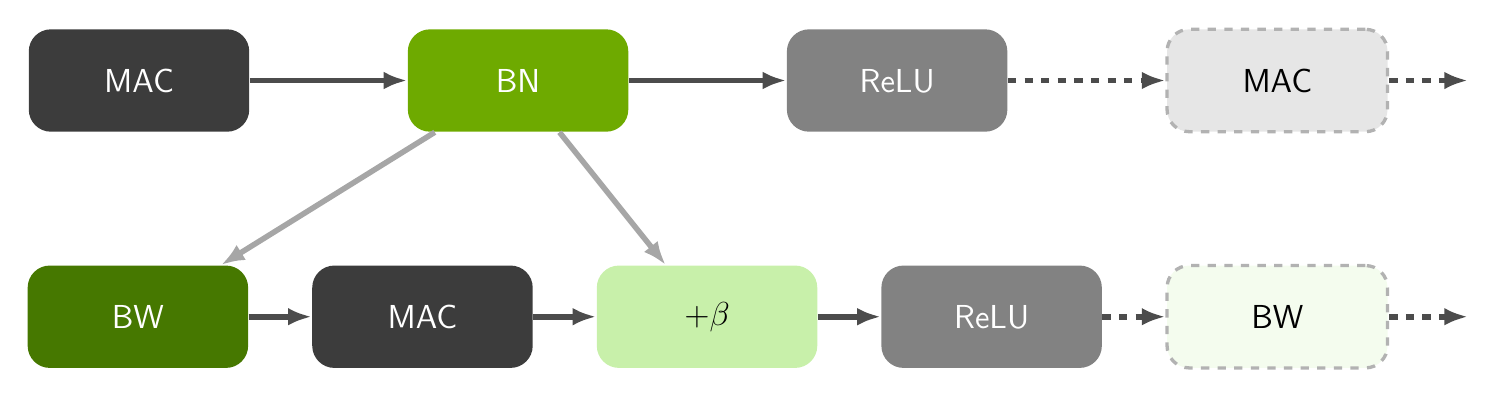
\begin{tikzpicture}[
  font=\large\sffamily,
  box/.style={
    rounded corners=8pt,
    minimum width=2.8cm,
    minimum height=1.3cm,
    align=center
  },
  solidbox/.style={box, draw=none},
  dashedbox/.style={box, draw=gray!60, dashed, very thick},
  arrow/.style={-{Latex[length=3mm]}, line width=2pt, draw=gray!70},
  blackarrow/.style={-{Latex[length=3mm]}, line width=2pt, draw=black!70},
  dashedblackarrow/.style={-{Latex[length=3mm]}, line width=2pt, draw=black!70, dashed},
]

% Top row
\node[dashedbox, fill=macgray] (macTopL) at (0,3) {MAC};
\node[solidbox, fill=relugray, text=white] (reluL) [left=2.0cm of macTopL] {ReLU};
\node[solidbox, fill=bngreen, text=white] (bn) [left=2.0cm of reluL] {BN};
\node[solidbox, fill=macdark, text=white] (macBotL) [left=2.0cm of bn] {MAC};

% Bottom row. The length x between rectangles: x = 2.8*4 + 2.0*3 - 2.8*5 = 0.8
\node[dashedbox, fill=bwlightL] (bwTop) at (0,0) {BW};
\node[solidbox, fill=relugray, text=white] (reluR) [left=0.8cm of bwTop] {ReLU};
\node[solidbox, fill=bwlight, text=black] (beta) [left=0.8cm of reluR] {$+\beta$};
\node[solidbox, fill=macdark, text=white] (macR) [left=0.8cm of beta] {MAC};
\node[solidbox, fill=bwdark, text=white] (bwBot) [left=0.8cm of macR] {BW};

% Arrows from BN
\draw[arrow] (bn) -- (beta);
\draw[arrow] (bn) -- (bwBot);

% Arrows between layers - top row
\draw[blackarrow] (macBotL) -- (bn);
\draw[blackarrow] (bn) -- (reluL);
\draw[dashedblackarrow] (reluL) -- (macTopL);
\draw[dashedblackarrow] (macTopL.east) -- ++(1.0cm,0);

% Arrows between layers - bottom row
\draw[blackarrow] (bwBot) -- (macR);
\draw[blackarrow] (macR) -- (beta);
\draw[blackarrow] (beta) -- (reluR);
\draw[dashedblackarrow] (reluR) -- (bwTop);
\draw[dashedblackarrow] (bwTop.east) -- ++(1.0cm,0);

\end{tikzpicture}